\documentclass{elsart}
\usepackage{graphicx,natbib,amssymb}

\journal{Software and Systems}

\begin{document}
\begin{frontmatter}

\title{A Design Rule Language for Aspect-oriented Programming}

\author[UFPE]{Rodrigo Bonif\'{a}cio\corauthref{cor}},
\corauth[cor]{Corresponding author.}
\ead{rba2@cin.ufpe.br}
\author[UFPE]{M\'{a}rcio Ribeiro},
\ead{mmr3@cin.ufpe.br}
\author[UFPE]{Marcos D\'{o}sea},
\ead{mbd@cin.ufpe.br}
\author[UFPE]{Alberto Costa Neto},
\ead{acn@cin.ufpe.br}
\author[UFPE]{Paulo Borba},
\ead{phmb@cin.ufpe.br}
\author[UPE]{S\'ergio Soares}
\ead{sergio@dsc.upe.br}
\address[UFPE]{Informatics Center, Federal University of Pernambuco, Recife,
Brazil}
\address[UPE]{Department of Computing and
Systems, University of Pernambuco, Recife, Brazil}


\begin{abstract}
FO Aqr is a close binary star in
which a magnetic white dwarf accretes from a cool companion. Light
curves and spectra show variations on the orbital frequency, the
white dwarf�s spin frequency and combinations of the two.
\end{abstract}

\begin{keyword}
Accretion, accretion disks \sep Line: profiles \sep
Binaries: close \sep Novae, cataclysmic variables
\PACS 97.10.Gz \sep 97.30.Qt \sep 97.80.Gm
\end{keyword}
\end{frontmatter}

\section{Introduction}
The support for variation points enables product customization from a set of
reusable assets~\cite{Pohl:2005aa}. However, variability management, due to its
inherent crosscutting nature, is a common challenge in software product line
(SPL) adoption~\cite{Clements:2001aa,Pohl:2005aa}. First, nontrivial features
often require associated variation points to be scattered through SPL artifacts.
Second, some approaches include product variant and configuration information
inside artifacts. Both problems can be observed for use case scenario
specifications.

Several authors have proposed the use of \emph{aspect-oriented} mechanisms to
better modularize the specification of crosscutting
concerns~\cite{Moreira:2004aa,Chitchyan:2007aa}. These techniques minimizes the
first problem, since they can be used to modularize the specification of certain
features. However, they do not support the different sources of variability that
occur in SPL requirements. With respect to the second problem, existing
approaches~\cite{Bertolino:2003aa,Eriksson:2005aa} proposed to
scenario variability management do not offer a clear separation between
variability management and scenario specification. As a consequence, in the case
where details about product variants are tangled with use case scenarios, the
removal of one variant from the product line requires changes to all related
scenarios. In summary, it is difficult to evolve both representations.

So in this paper we go beyond the common-variant scenario composition issues and
consider a more encompassing notion of variability management, including
artifacts such as feature models~\cite{Gheyi:2006aa,Czarnecki:2000aa} and
configuration knowledge~\cite{Czarnecki:2000aa,Pohl:2005aa}. We explain this as a
crosscutting phenomenon, using Masuhara and Kiczales work~\cite{Masuhara:2003aa},
and apply this view of \emph{variability management as crosscutting} for
modularizing SPL use case scenarios, providing the necessary separation between
variability and scenario specification concerns. We also formalize the derivation
of product specific scenarios in our approach, as demanded by current SPL
generative practices~\cite{Krueger:2006aa}. This formalization is based on our
framework for modeling the composition process of scenario variabilities with
feature models, product configuration, and configuration knowledge. Besides
supporting the mentioned separation of concerns, this framework helps to
precisely specify how to weave the different representations in order to generate
specific scenarios for a SPL member. Therefore, the main contributions of this
work are the following:

\begin{itemize}
\item Characterization of the languages of variability management as a
crosscutting concern and, in this way, proposing an approach where variability
concerns are separated from other concerns (Section~\ref{sec:svmc}).

%Although this work focus on requirement artifacts, more specifically use case scenarios, we argue that such separation is also valid for other SPL artifacts. Actually, it has already been claimed for source code~\cite{Alves:2006aa,Apel:2006aa}, without considering the importance of variability artifacts.

\item A framework for modeling the composition process of scenario variability
mechanisms (Section~\ref{sec:modeling-framework}). Differently from existing
works~\cite{Morin:2008aa,Groher:2008aa}, this framework gives a basis for
describing variability as crosscutting mechanisms, at the same time it considers the contribution of different input
languages: feature models, product configuration, configuration knowledge and SPL use case
model. Moreover, the reference implementation provided for each variability
mechanism corresponds to the essencial parts of a tool environment for scenario
variability management. In this paper we focus just in these essencials.

\item Specification of three {\color{red}sources of variability for use case
scenarios: variability in function (Section~\ref{sub:pd-weaver}),
variability in data (Section~\ref{sub:bind-weaver}), and variability in control
flow (Section~\ref{sub:sc-weaver})}. This specification provides a more formal
semantic representation when compared to existing works; which is an important property
for supporting the automatic derivation of product specific artifacts.
\end{itemize}

{\color{red}The sources of
variability (or kinds of composition) for use case scenarios presented here are
not complete. However, our modeling framework is able to represent
other interesting sources of variability, such as context-aware adaptability.
Additionally, since the word \emph{scenario} has different meanings in software
engineering, we want to make clear that in the remainder of this paper the term
\emph{scenario} corresponds to textual use case scenarios. We explain the structure
used for specifying scenarios in Section~\ref{sub:spl-uc}}.

Since our concept of crosscutting mechanism is based on Masuhara and Kiczales
work~\cite{Masuhara:2003aa}, a smaller contribution of this paper is to apply
their ideas to the languages of variability management,  reinforcing the
generality of their model, which was originally instantiated only for mechanisms
of aspect-oriented programming languages. Based on their view of crosscutting, we
can reason about variability management as a crosscutting concern that involves
different input specifications that contribute to derive a specific member of a
given SPL. 

Finally, we evaluate our approach (Section~\ref{sec:evaluation}) by comparing it
to alternative approaches using different product lines. We also relate our work
with other research topics (Section~\ref{sec:related}) and present our concluding
remarks (Section~\ref{sec:conclusions}). 
\section{Motivation Problem}

The concept of modularity applied to software development was first
introduced by Parnas~\cite{parnas-on_the_criteria-cacm1972}. Such
concept is still used as a guide for architects and is being applied
in another areas. Modularity is closely related to design decisions
that decompose and organize the system into a set of modules. The
following qualities attributes are expected in a modular design:

\begin{description}

\item[Comprehensibility] A modular design allows developers to
understand a module looking only at: (1) the implementation of the
module itself; and (2) the interfaces of the other modules
referenced by it\footnote{This comprehensibility degree is also
known as \emph{modular reasoning}.}.

\item[Changeability] A modular design enables local
changes. If changes are necessary in the internal implementation of
a module \emph{A}, the other modules that depend exclusively on
\emph{A's interface} will not need to change, since there is no
modification in the module interface.

\item[Parallel development] After the specification of the module
interfaces, a modular design enables the parallel development of
modules. Different teams might only focus in their own modules
development, reducing the time-to-market and the need of
communication.

\end{description}

Parnas proposed the \emph{information hiding} principle as the
criteria to be used in decomposition of systems into modules.
According to Parnas, the parts of a system that are more likely to
changes must be hidden into modules with stable interfaces.

Aspect-Oriented Programming was proposed to modularize crosscutting
concerns. However, constructions supported by
AspectJ~\cite{kiczales-CACM2001} like languages can produce high
coupling between the base code and the aspects, which may compromise
the aforementioned modular criteria. In this section, we illustrate
this problem through some examples.

\subsection{Example 1}

Suppose the requirement of synchronizing (concurrency management)
all methods of a class. Such requirement consists of encompassing
with synchronized blocks the bodies of all methods.
Listing~\ref{lst:ao-synchronizing} illustrates an implementation of
this concern in AspectJ applied to the \emph{EmployeeRepository}
class.

\scriptsize
\begin{lstlisting}[frame=single, caption={Aspect responsible for implementing the concurrency concern.},label=lst:ao-synchronizing, language=Java]
public aspect SynchronizationAspect {

    Object around(Object o): this(o)
            && execution(* EmployeeRepository.*(..)) {
        synchronized(o) {
            return proceed(o);
        }
    }
}
\end{lstlisting}
\normalsize

Now, suppose a new feature intended to count the number of employees
registered in a given profile. Such feature might be implemented as
a new method in the \emph{EmployeeRepository} class
(Listing~\ref{lst:new-method}).

\scriptsize
\begin{lstlisting}[frame=single, caption={A new method for counting the number of Employees.},label=lst:new-method, language=Java]
public class EmployeeRepository {

    public void insertEmployee(Employee employee) { ... }

    public void removeEmployee(Employee employee) { ... }

    public int getNumberOfEmployees(Profile profile) {
        // Business logic to count the number of Employees
    }

}
\end{lstlisting}
\normalsize

If a class developer oblivious about the
\emph{SynchronizationAspect} aspect decides to implement the
\emph{getNumberOfEmployees} method, at least three problems can
occur:

\begin{enumerate}

    \item the \emph{getNumberOfEmployees} method created by the class
    developer might not need concurrency management, but it will be
    synchronized by the aspect;

    \item if the class developer, oblivious about the aspect,
    implements concurrency management in the \emph{getNumberOfEmployees} method,
    such method would be synchronized twice; and

    \item depending on how the synchronization approaches are implemented
    by the aspect and class developers, together they might lead the system
    to a dealock or a livelock situation~\cite{lea-java-coop-1999}.

\end{enumerate}

In such cases, the expected behavior of the system could be
compromised, since some additional synchronization would be created
or, even worst, the system might reach a dealock or a livelock.

The situation above exposes that problems of modularity have
occurred: (1) the comprehensibility is compromised, since two
modules should be studied in order to understand the concern; and
(2) the parallel development is problematic, because one developer
can implement unintended behavior into a module which, although it
is not under his responsibility, might break the system.

In summary, we conclude that any unanticipated change in the class
may cause problems and the application might not behave as presumed.
Notice that we have a cyclical dependency situation: the aspect
depends on the class syntactically; and to change the class, the
developer must be aware about the aspect.
Figure~\ref{dsm:concurrency} illustrates such cyclical
dependency through a DSM (presented in Section~\ref{}), whereas
Figure~\ref{dsm:concurrency-drs} shows design rules coming into
play to remove the dependency between the aspects and class.

\begin{figure}[h]
    \begin{center}
        \subfigure[Cyclical Dependency between an aspect and a class.] {
            \begin{scriptsize}
            \begin{tabular}{|l|l|l|l|} \hline
                  &                             & 1     & 2     \\ \hline
                1 & SynchronizationAspect.aj    & \paintcell     & x     \\ \hline
                2 & EmployeeRepository.java     & x     & \paintcell      \\ \hline
            \end{tabular}
            \end{scriptsize}
            \label{dsm:concurrency}
        }
        \subfigure[Design Rules removing Cyclical Dependency.] {
            \begin{scriptsize}
            \begin{tabular}{|l|l|l|l|l|} \hline
                  &                             & 1     & 2    & 3 \\ \hline
                1 & Design Rules                &       &      &   \\ \hline
                2 & SynchronizationAspect.aj    & x     &      &   \\ \hline
                3 & EmployeeRepository.java     & x     &      &   \\ \hline
            \end{tabular}
            \end{scriptsize}
            \label{dsm:concurrency-drs}
        }
        \caption{Concurrency concern with/without Design Rules.}
    \end{center}
\end{figure}

\subsection{Example 2}

Another example of modularity issue might arise when a team is
assigned to develop a crosscutting concern and another team is
assigned to develop the base concerns of a system. In order to
reduce the time to market, it may be desirable to develop both
concerns in parallel. However, without the use of a clear interface
between those concerns, a lot of communication might be required,
which, in fact, compromises the parallel development.

When reasoning about modularity in software engineering,
the benefit of parallel development is frequently not considered. Even after
Parnas has claimed that modularity is more than program structure. Actually,
his view of modularity is related to the assignment of development
activities, which, of course, may be reflected in the program
structure~\cite{parnas-icse-03}.

\begin{quote}\emph{
My early work clearly treated modularisation as a design
issue, not a language issue. A module was a work assignment,
not a subroutine or other language element. Although
some tools could make the job easier, no special tools were
needed to use the principal, just discipline and skill.}
(D. Parnas)
\end{quote}


% include the parnas review of modularity
% read a bit more about the steimann discussion on AOP modularity
% we need a clear interface for both aspect and base code....

A similar view of modularity was presented by Baldwin and
Clark~\cite{clark-design-rules-book}. They proposed a theory that
considers a \emph{modular design} as a key factor for innovation in
different domains (hardware, software, and so on). Moreover, they
observed that a modular design reduces the communication paths among
design decisions, in such a way that unities of work can be developed
in parallel.

For instance, supposing that a team is responsible for developing
the use cases related to the \emph{complaint management} concern (a core concern
of Health Watcher system~\cite{soares-oopsla-02}); and another team is responsible
for an auditing concern that must be triggered whenever a change in a
complaint occurs. Without a clear interface stating which are the relevant
complaint changes (the set of join-points) and how these join-points should be
written by the complaint management team, any increment in the core concern
must be communicated to the auditing team. Consequently, it is difficult to
implement the auditing concern at the same time that the complaint management
concern is being developed. Although these concerns can be encapsulated in
single unities, there is no modular design in this case.

We can represent this kind of dependence by means of Design Structure
Matrices (DSMs). DSMs are used to visualize dependencies among design
parameters, which correspond to any decision that needs to be made along the
product design. Parameters are disposed in both rows and columns of a matrix.
The notion of dependency, represented as a 'x' mark in the matrices, arises
whenever a design decision depends on another. For
instance, consider the DSM depicted in Figure~\ref{dsm:hw01}, which represent
some design parameters and respective dependencies of the Health Watcher
system. Based on this DSM, we can realize that decisions regarded to the
complaint implementation (row 5) depends on decisions about complaint
requirements (dependence row 5, column 2), about architectural
decisions~\footnote{Examples of architectural decisions for the Health Watcher
system are the selected style (layers), patterns, and technologies for each
layer or concern (presentation, distribution, persistence, and so on)}
(dependence row 4, column 4), and about the auditing concern (dependence row 4,
column 6). This last dependency occurs because the team responsible for developing
the \emph{complaint concern} have to know how to develop the extension points for
the \emph{auditing concern}. Moreover, as we can observe in
Figure~\ref{dsm:hw01}, the auditing implementation also depends on the
complaint implementation decisions, since changes in its implementation should
be notified to the auditing implementation team. In this way, there is a
cyclical dependency between complaint implementation and auditing
implementation -- a clear example of non modular design.

\begin{figure}[htb]
\centering
\begin{scriptsize}
\begin{tabular}{|l|l|l|l|l|l|l|l|} \hline
  &                             & 1     & 2     & 3     & 4     & 5     & 6 \\ \hline
1 & Goals and constraints       &       &       &       &       &       &   \\ \hline
2 & Complaint requirements      & x     &       &       &       &       &   \\ \hline
3 & Auditing requirements       & x     &       &       &       &       &   \\ \hline
4 & Architectural decisions     & x     & x     &       &       &       &   \\ \hline
5 & Complaint implementation    &       & x     &       & x     &       & x \\ \hline
6 & Auditing AO implementation  &       &       & x     &       & x     &   \\  \hline
\end{tabular}
\end{scriptsize}
\caption{DSM Analysis Health Watcher}
\label{dsm:hw01}
\end{figure}


Based on the information hidden principle, we should encapsulate the
dependences between complaint and auditing concerns in a special kind
of interface (a design rule). Design rules establish strict partitions
of knowledge and effort at the outset of a design process.
They are not just guidelines or recommendations: they must be rigorously
obeyed in all phases of design and production~\cite{clark-design-rules-book}.
Applying design rules to our current example, we improve the design structure
by removing the cyclical dependencies between complaint and auditing concerns.
The reviewed DSM is presented in Figure~\ref{dsm:hw02}. Notice that a new parameter
(actually a design rule) was introduced (row 4) and all dependencies are bellow
the main diagonal (there is no more cyclical dependencies).

\begin{figure}[htb]
\centering
\begin{scriptsize}
\begin{tabular}{|l|l|l|l|l|l|l|l|l|} \hline
  &                                 & 1     & 2     & 3     & 4     & 5     & 6 & 7 \\ \hline
1 & Goals and constraints           &       &       &       &       &       &   &   \\ \hline
2 & Complaint requirements          & x     &       &       &       &       &   &   \\ \hline
3 & Auditing requirements           & x     &       &       &       &       &   &   \\ \hline
4 & Architectural decisions         & x     & x     &       &       &       &   &   \\ \hline
5 & Auditing design rule            &       & x     &   x   &       &       &   &   \\ \hline
6 & Complaint implementation        &       & x     &       &   x   & x     &   &   \\ \hline
7 & Auditing AO implementation      &       &       &   x   &       & x     &   &   \\ \hline
\end{tabular}
\end{scriptsize}
\caption{DSM Analysis Health Watcher}
\label{dsm:hw02}
\end{figure}


This idea of defining interfaces between aspect code and adviced code is not
really new. Next, we present some proposals to solve this problem and discuss
how our approach improve existing works.

\subsection{Existing solutions}

% ok, o problema realmente existe. mas ele n�o � novo. precisamos discutir que
% existem propostas para esse problema. Por outro lado elas n�o atendem.
% Possivelmente, um caminho � a id�ia de que design-rules precisam ser
% rigorosamente seguidas. Sempre tenho d�vidas em rela��o a essa palavra:
% ``rigorosamente''

\subsubsection{Open Modules}

Open Modules is an approach for dealing with modularity issues in 
AOP~\cite{aldrich-ecoop-05}. Besides exposing data structures and 
functions, Open Modules' interfaces can also expose pointcuts denoting 
internal semantic of events. Clients of these modules are able to advice 
only exported pointcuts. Moreover, by exporting a pointcut, the module's 
developer is compromised to maintain the semantics of that pointcuts, 
which, in fact, mitigates the fragile pointcut problem. 

However, Open Modules do not offers mechanims for describing which 
are the responsabilities of aspect developers. As a consequence, 
module developers are still able to implement part of a concern 
assigned for a different team and they can not assume the existence 
of any behavior expected to be modularized as an aspect. 

For instance, consider the implementation of a mobile
game product line. Listing~{lst:paint-method} presents part of 
a non-variant code responsible for painting graphical elements 
on the screen. Methods \emph{paintBeforeScrolling} and
paintScolling are introduced (by means of intertype declararions),
and represent variation points that should be implemented as aspects for each 
target device. Open Modules does not specify that such methods must be called 
within the \emph{paint} method and that they must be introduced by aspects. Although
not so common, base code calling methods introduced by aspects are presented 
in several examples~\cite{eide-aosd-08}. Therefore, it is necessary to define which 
methods are expected to be introduced by aspects.

\scriptsize
\begin{lstlisting}[frame=single, caption={Dependency of a base code to an aspect code.},label=lst:paint-method, numbers=left, language=Java]
 public void paint(Graphics g) {
	Enemy myEnemy = null;
	int i = 0;
	int j = 0;
	g.setClip(0, 0, Resources.CANVAS_WIDTH, Resources.CANVAS_HEIGHT);
	paintBeforeScrolling(g);
	if (this.scroll.isScrolling) {
	 	paintScrolling(g);
	} else if (!isGameOver){
	 ...
\end{lstlisting}

\normalsize

\subsection{Aspect Box}

\subsubsection{XPIs}

The Crosscut Programming Interfaces (XPIs) is one attempt for defining design rules between aspects and 
advised code~\cite{sullivan-sigsoft-2005,sullivan-ieee-sw-2006}. Such interfaces specify which are the exposed 
join-points of a base code. Although an abstract XPI representation was provided in~\cite{sullivan-sigsoft-2005}, Griswold et. al  
presented how to implement crosscutting interfaces as syntactic constructs of AspectJ~\citet{sullivan-ieee-sw-2006}. 
Based on this approach, design rules are documented using \emph{abstract pointcut descriptions} and constraints 
applied to the base code. These constraints might be written as \emph{declare warning} (or \emph{declare error}) constructs
or just as comments in the source code (when a constraint can not be expressed as a \emph{declare warning} 
or \emph{declare error}). 

XPIs authors argue that one interesting characteristic of the approach is that it is does not require any new construct in 
the AspectJ language. In fact, this characteristic encourage the use of this approach in environments that are already 
using the AspectJ language. However, most of the constraints required for defining the responsibilities of both 
class developers and aspect developers can not be checked using the proposed XPI language. Consequently, it is not possible 
to guarantee, at least automatically, if all design rules are being obeyed. For instance, we can not express using AspectJ constructs 
that a call to a method must occurs within the flow of another method. Actually, we can define such pointcut, but if it does not exist, no 
error is reported. 


  

\section{A language for specifying AO design rules}
\label{sec:drlang}

%XXX CRIAR FIGURA COM O META-MODELO S� COM O LADO ESQUERDO E COLOCAR NO DIRETORIO
%XXX Incluir a nova BNF?
%XXX Criterios de matching
%XXX Implementacao atual usando ABC
%XXX Discutir a implementacao explicita da interface por ambos

In this section we present the \emph{Language for Specifying
Design Rules (LSD)}. The main objective of this language is to
decouple syntactically and semantically classes and aspects,
maximizing independent development opportunities. Through the
definition of Design Rules we argue that both class and aspect
developers can work independently if a minimum set of constraints
is defined and respected.

LSD was defined as a way of expressing clearly and unambiguously
design rules established during all development phases, specially
during software design. The language serves as a mechanism for
creating more modular software, because it decouples classes and
aspects through the establishment of the minimum requirements to
their parallel development.

The initial motivation for the language development was improving
modularity of aspect-oriented systems. However, other design
rules, like those defined during architectural design, can be
naturally expressed by the language.

On the other hand, its utilization requires the creation of new
artifacts to contain design rule specifications. Also, in order to
define appropriate design rules its expected that software
designers have enough experience for that. Additionally,
developers must get used to new language constructs. In spite of
that, explicitly expressing the design rules, and specially being
capable of verifying them, makes easy the task of developing new
components.

% comparar com uma documenta��o textual

In this section we present LSD main constructs, based on previous
work... %~cite\{DoseaLAWASP}.

\subsection{LSD overview}
\label{sec:lsdoverview}

%---------------------------------------------

Many Object-Oriented programming languages provide the concept of
interface which specify a public set of methods and constants
obligatorily provided by any class that declares to implement it.
This interface notion allows developers to create separated and
narrow interfaces to different clients of the same class, limiting
the coupling between them.

Our concept of interface, which we call a \emph{Design Rule}, is
wider. A Design Rule contains a set of constraints that must be
followed by components that declare to implement them. These
constraints are automatically verified by a tool that points out
when some constraint is disrespected by class and aspect
developers.

Figure~\ref{fig:meta-model} shows the Design Rules specification
language meta-model. A rule description is composed by one or more
structural rules (section~\ref{sec:structuralrules}). They are
used to define structural constraints for classes and aspects.
Thus, a class can define fields, method signatures and behavioral
rules. These behavioral rules (section~\ref{sec:behavioralrules})
can be defined within classes and aspects scope or within their
methods and advices (only aspects).

\begin{figure}[htp]
  \begin{center}
  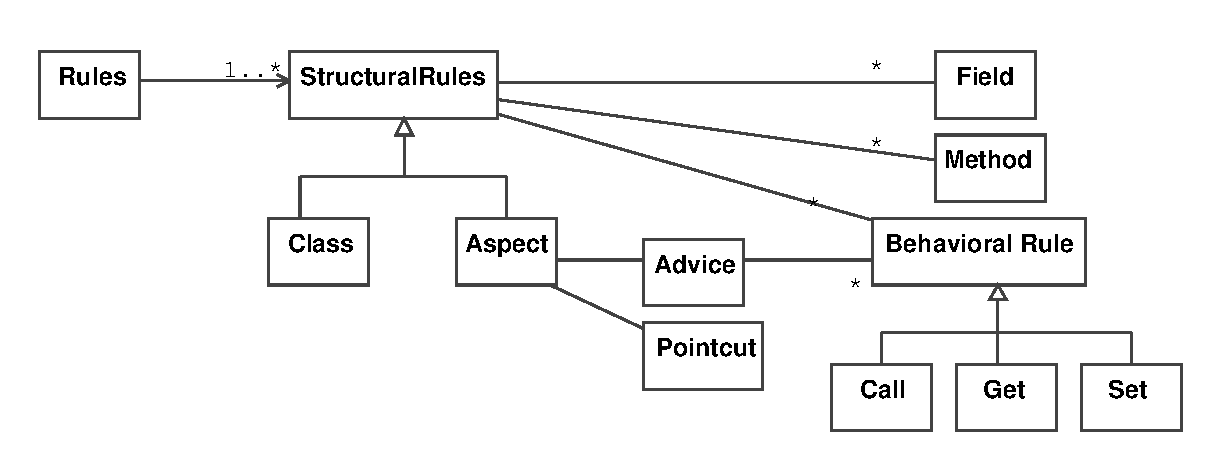
\includegraphics[width=1.0\textwidth]{images/meta-model.eps}\\
  \caption{Design Rule Language and Configuration Module Meta-Models}
  \label{fig:meta-model}
  \end{center}
\end{figure}

\subsection{Structural Rules}
\label{sec:structuralrules}

Structural Rules are design rules that describe constraints about
members of classes and aspects. Their format is similar to the
interface description in Java~\cite{JAVA}, but it is possible to
include additional constraints (beyond required public methods and
constants), like attributes that must be declared and required
method visibility. Besides, there are specific constraints about
aspects structure, like requiring an specific pointcut declaration
and/or advice.

Listing~\ref{lst:dr1} shows examples of structural rule
descriptions to be respected by classes and aspects. Line 1
contains the declaration of the \texttt{System} design rule that
aggregates a set of \emph{structural rules}. Following, it appears
the \emph{structural rule} declaration for
\texttt{ComponentRecord} to be respected by classes. It requires
the declaration of two methods with compatible signatures (Lines
2-5). There is also the \texttt{Component} \emph{structural rule}
(Lines 6-8), which must be respected by classes. The last
\emph{structural rule} declared (Lines 9-16), called
\texttt{TransactionalManagement} must be followed by aspects,
which must contain a pointcut \texttt{service} and the
\emph{advices before} and \emph{around} to this pointcut.

\scriptsize
\begin{lstlisting}[frame=single, caption={Structural Rule for Transaction Management.},label=lst:dr1,
                numbers=left,
                language=Java,
                morekeywords={dr, aspect, pointcut}]
dr System {
    class ComponentRecord {
        public void insert(Component c);
        public void delete(Component c);
    }
    class Component {
        int key;
    }
    aspect TransactionalManagement {
      pointcut service(): execution(ComponentRecord.insert(Component)) ||
                          execution(ComponentRecord.delete(Component));
      before(): service() {
      }
      after(): service() {
      }
    }
}
\end{lstlisting} \normalsize


\texttt{System} design rule declares the minimum requirements so
that components \texttt{ComponentRecord}, \texttt{Component} and
\texttt{TransactionalManagement} can be developed in parallel. So,
for example, the \texttt{ComponentRecord} developer needs to know
only that it must implement methods \texttt{insert} and
\texttt{delete} so that other components works correctly. The
language enables the specification of \emph{structural rules} to
attribute declaration, useful in cases that clients of the
component requiring it. An example of it appears in
Listing~\ref{lst:dr1} within the \texttt{Component}
\emph{structural rule}. It requires that Component classes provide
an \texttt{attribute} int called \texttt{key}.


\subsection{Behavioral Rules}
\label{sec:behavioralrules}

A \emph{behavioral rule} provides a mechanism for specifying
constraints about the behavior of components. When a behavioral
rule is defined within the scope of a class or aspect it means
that it has to be respected at any place, for example, if a rule
\emph{call} is used within the scope of a class, it means that the
required method must be called at least once in this class.
Another example is requiring a read (or write) of an specific
attribute within a certain scope.

The Table~\ref{tbl:commands} shows the \emph{behavioral rules}
provided by the language. The scope of these rules includes
classes, aspects, methods and advices. Every rule initiated by 'x'
guarantees that the rule will be followed only in the defined
scope and this will not be possible in any other location. For
example, the \emph{xcall} rule guarantees that an specific method
will be called exclusively within the scope in which it was
defined. Calls outside the scope are not allowed. In case that the
rule \emph{xcall(method)} exists in more than one scope for the
same method, then this call can only occur within these defined
scopes.

\begin{table}
  \centering
  \caption{Behavioral Rules provided by the LSD.}\label{tbl:commands}
    \begin{tabular}{|c|p{10.5cm}|}
      \hline
      \textbf{Rule} & \textbf{Description}\\
      \hline
      \emph{call(method)} & It must have a call to the method passed as parameter within the defined scope.\\
      \hline
      \emph{xcall(method)} & It must have a call to the method passed as parameter exclusively in the defined scope.\\
      \hline
      \emph{set(attribute)} & It must have an state change on the attribute passed as parameter within the defined scope.\\
      \hline
      \emph{xset(attribute)} & It must have an state change on the attribute passed as parameter exclusively within the defined scope.\\
      \hline
      \emph{get(attribute)} & It must have an state access to the attribute passed as parameter within the defined scope.\\
      \hline
      \emph{xget(attribute)} & It must have an state access to the attribute passed as parameter exclusively within the defined scope.\\
      \hline
    \end{tabular}
\end{table}

These rules are also useful to guarantee, for example, that a
method must not be called in a given scope, by using the negation
operator (!). When a \emph{behavioral rule} is defined within the
scope of a class or aspect, it is valid for the entire class. One
\emph{call} within a class indicates that at some point of the
class that call must occur.

\scriptsize
\begin{lstlisting}[frame=single, caption={Behavioral Rules for Transaction Management.},
                   label=lst:dr2, numbers=left, language=Java,
                   morekeywords={dr, xcall, aspect, pointcut} ]
dr System {
    class ComponentRecord {
        public void insert(Component c);
        public void delete(Component c);
    }
    class Component {
        int key;
    }
    class Persistence {
        void beginTransaction();
        void endTransaction();
        void openConnection();
        void closeConnection();
    }
    aspect TransactionalManagement {
      pointcut service(): execution(ComponentRecord.insert(Component));
      before(): service() {
          xcall( Persistence.beginTransaction() );
      }
      after(): service() {
          xcall( Persistence.endTransaction() );
      }
   }
}
\end{lstlisting} \normalsize

Listing~\ref{lst:dr2} shows the using of the \emph{xcall
behavioral rule} (Lines 18 and 21). These two rules indicate that
methods must be called exclusively within the advice scope,
prohibiting calls from any other place among the components
specified by the design rule \texttt{System}. For example, if the
method \texttt{Persistence.beginTransaction()} was called from the
\texttt{delete} method of the class that implement the
\texttt{ComponentRecord} \emph{structural rule} an error would be
presented to the user. Thus, through simple rules it is possible
to improve system modularity, documenting the interaction rules
between components and guaranteing that they are being followed by
using a verifier. It is important that classes and aspects always
implement the \emph{design rules} documented by the software
designer. If this is not done, it is impossible to guarantee that
they will be respected. For example, a class that implements no
\emph{structural rules} defined by the \texttt{System}
\emph{design rule} can call the method
\texttt{Persistence.beginTransaction()}, even if in the
architecture project this call should only occur within the aspect
responsible for transaction management.

%-------------------------------

\subsection{Explicit implementation of Design Rules}
\label{sec:explicitimpldr}

Trying to keep similarity with Java interfaces concept, and
following the LSD principle of establish an interface between
classes and aspects, LSD requires that both class and aspect
explicitly implements the design rules.

In order to developers being aware of the design rules they must
respect, the components being developed must include the name of
all design rules that it implements in the \emph{implements
clause} like classes that implement ordinary interfaces.
Additionally, for each implemented design rule, it must be provide
the name of one or more the structural rules.

Thus, if the class developer needs to make a change, it is easier
to identify which design rules must be respected, facilitating
evolution some jobs and preventing some errors. Besides, its use
enables automatic verification and separate compilation. The using
of \emph{implements} obligates a class or aspect to follow all the
rules defined by the corresponding \emph{structural rule}.

\scriptsize
\begin{lstlisting}[frame=single, caption={Explicit implementation of the Design Rule System.},
                   label=lst:comp1,
                   numbers=left, language=Java,
                   morekeywords={dr, xcall, aspect, pointcut}]
class UserRecord implements System(ComponentRecord) {
    ...
}

class User implements System(Component) {
    ...
}

class Persistence implements System(Persistence) {
    ...
}

aspect TransactionalManagement implements
System(TransactionalManagement) {
    ...
}
\end{lstlisting} \normalsize

Listing~\ref{lst:comp1} shows examples of components that follows
the \emph{design rule} \texttt{System}. For example, classes
\texttt{UserRecord} (Lines 1-3), \texttt{User} (Lines 5-7) and
 \texttt{Persistence} (Lines 9-11) indicate the names of their corresponding \emph{structural rules},
\texttt{ComponentRecord}, \texttt{Component} and
\\texttt{Persistence}, respectively. In an identical form, aspect
\texttt{TransactionalManagement} (Lines 13-16) implements
\texttt{System} and the corresponding \emph{structural rule}
\texttt{TransactionalManagement}.


\subsection{Additional constraints}
\label{sec:additionalconstraints}

Previous sections discussed the general idea of the LSD. In this
section we present more language constructs that provide ways of
expressing additional constraints.

\subsubsection{Modifiers}

The first one of them is related to components modifiers. It might
be necessary that a certain class, for example, have public and
not package visibility.

Listing~\ref{lst:drmodifiers} shows part of the design rule
\texttt{System}. \texttt{ComponentRecord} requires that classes
that implement the design rule \texttt{System} are \texttt{public}
classes and provide two \texttt{public} methods with a
\texttt{void} return type and with a parameter \texttt{Component}.
Others modifiers are accepted, like \texttt{final},
\texttt{synchronized} and \texttt{abstract}, since the language is
focused on specifying the minimum requisites about the component
structure.

\scriptsize
\begin{lstlisting}[frame=single, caption={Modifiers constraints.},
                   label=lst:drmodifiers, numbers=left, language=Java,
                   morekeywords={dr, xcall, aspect, pointcut} ]
dr System {
    public class ComponentRecord {
        public void insert(Component c);
        public void delete(Component c);
    }
    public class Component {
        private int key;
    }
    ...
}
\end{lstlisting} \normalsize

Additionally, listing~\ref{lst:drmod} contains a
\texttt{Component} class that must be \texttt{public}. Also, it
must provide a \texttt{private} attribute called \texttt{key} of
\texttt{int} type. It might be strange to define a constraint
about a private part of a class, but sometimes aspects need to
refer to private parts of classes. If this dependency is defined
in a design rule, it is possible to explicitly express it.

\subsubsection{Implements/Extends}

Another interesting type of constraint is to require that the
class implementing a certain \emph{structural rule} implements or
extends an specific type.

An example of this constraint is shown in
Listing~\ref{lst:drimpext}. Classes that implement the structural
rule \texttt{ComponentRecord} must explicitly implement the
interface \texttt{BaseRecord}. Following, the structural rule
\texttt{Component} must extend directly class
\texttt{BaseComponent}.

% BaseRecord � uma interface real? Est� definida na Design Rule?
% Implements em Interfaces para declarar que implementa uma DR?
% Discutir melhor as op��es de implements nas classes, m�dulo com mapeamento e anota��es

\scriptsize
\begin{lstlisting}[frame=single, caption={Implements/Extends constraints.},
                   label=lst:drimpext, numbers=left, language=Java,
                   morekeywords={dr, xcall, aspect, pointcut} ]
dr System {
    public class ComponentRecord implements BaseRecord {
        public void insert(Component c);
        public void delete(Component c);
    }
    public class Component extends BaseComponent {
        private int key;
    }
    ...
}
\end{lstlisting} \normalsize


\subsubsection{Inter-type declarations}

Inter-type declarations enable aspects to introduce attributes and
methods in classes. At the same time that it is an interesting
mechanism, it may create dependencies between classes and aspects.
This mechanism is frequently used in aspect-oriented software
product lines to introduce variable method implementations or
attributes values in classes. Design rules can be used to
explicitly create a contract between classes and aspects
introducing the variabilities.

Listing~\ref{lst:dritd} shows a design rule
\texttt{ScreenAtributtes} that declares two structural rules:
\texttt{MainScreen} and \texttt{SizeVariability}. The last one
must provide two inter-type declarations of fields \texttt{WIDTH}
and \texttt{HEIGHT} in the class that implement the structural
rule \texttt{MainScreen}. As a consequence, the class developer
can be sure that these two attributes will exist and can use it.

\scriptsize
\begin{lstlisting}[frame=single, caption={Implements/Extends constraints.},
                   label=lst:dritd, numbers=left, language=Java,
                   morekeywords={dr, xcall, aspect, pointcut} ]
dr ScreenAttributes {
    class MainScreen {
       ...
    }
    aspect SizeVariability {
        public static final int MainScreen.WIDTH;
        public static final int MainScreen.HEIGHT;
    }
}
\end{lstlisting} \normalsize

\subsection{Summary of constraints}
\label{sec:summaryofconstraints}

%-------------------------------
\subsubsection{Covered constraint types}

Covered Constraint Types

Required/Prohibited

Classes, Interfaces, Aspects

Fields, Methods, ITD, Advices, Pointcuts

Inheritance / Interface implementation

Method Calls

Attribute Get / Set


\subsubsection{Uncovered but planned constraint types}

Exceptions

Member Expressions

Class/Interface/Aspect Expressions

\subsection{LSD implementation}

LSD has an initial implementation using the ABC extensible
compiler for AspectJ~\ref{ABC}.

Descrever o ABC.

Descrever como o ABC foi estendido

Mostrar uma figura com o funcionamento logico do verificador.

Descrever alguma experiencia sobre a facilidade de extensao (ou
nao) do abc.

%XXX Implementacao atual usando


%---------------------------------------------
% PARTE DE ARTIGO ANTIGO


%In this section we present a Design Rule specification language.
%The main objective of this language is to decouple syntactically
%and semantically classes and aspects, maximizing independent
%development opportunities. Through the definition of Design Rules
%we argue that both class and aspect developers can work
%independently if a minimum set of constraints is defined and
%respected.
%
%\scriptsize
%\begin{lstlisting}[frame=single,
%                   caption={Display Update Design Rule.},
%                   label=lst:displayUpdateDR,
%                   numbers=left,
%                   language=Java,
%                   morekeywords={dr, xcall}]
%dr DRUpdateShape {
%    interface IShape {
%        void moveBy(int dx, int dy);
%    }
%
%    class Shape implements IShape {
%        void moveBy(int dx, int dy) {
%          xset(IShape+.*);
%        }
%    }
%
%    class Display {
%        void update();
%    }
%
%    aspect UpdateSignaling {
%        pointcut change():
%            execution( void IShape.moveBy(int, int) );
%
%        after() returning: change(){
%            xcall( void Display.update() );
%        }
%    }
%}
%
%\end{lstlisting}
%\normalsize
%
%Listing~\ref{lst:displayUpdateDR} contains a Design Rule
%specification for the Display Update concern shown in the section
%~\ref{sec:problem}. The Design Rule \emph{DRUpdateShape} enforces
%that it is necessary to define an interface \emph{IShape}
%containing at least the method \emph{moveBy} (Lines 2-4). Also,
%all classes acting as a \emph{Shape} must implement \emph{IShape}
%and state changes on attributes are allowed only within the
%\emph{moveBy} method (Lines 6-10). It also requires that a class
%\emph{Display} with a method \emph{update} must exist (Lines
%12-14). Additionally, it requires the existence of the aspect
%\emph{UpdateSignaling} with a pointcut \emph{change}. This
%pointcut must be referred by an \emph{after returning} advice that
%is the exclusive point, among the components specified by the
%Design Rule, allowed to call the method \emph{update} from class
%\emph{Display} (Lines 16-23).
%
%The Design Rule \emph{DRUpdateShape} specifies the minimum
%requisites that each component developer must know about the
%others, hence allowing their independent development. This
%specification uses a language similar to that used in the
%development of the components, making the specification much
%simpler. Comparing with Griswold \emph{et
%al}~\cite{griswold-xpi-ieee06} approach, it would be necessary
%approximately twice lines of code to specify the XPI, yet, many
%rules would still being expressed in natural language.
%
%The Listing \ref{lst:displayUpdateXPI} shows the Design Rules
%using the Griswold \emph{et al}~\cite{griswold-xpi-ieee06}
%approach. This approach allows only to check if the Design Rules
%are being followed, but requires from the class developer deep
%knowledge about AspectJ constructions, besides it does not guide
%developers. Our language supports the declarative specification of
%Design Rules adopting a syntax similar to the used by both
%developers.
%
%\scriptsize
%\begin{lstlisting}[frame=single,
%                   caption={Display Update XPI.},
%                   label=lst:displayUpdateXPI,
%                   numbers=left,
%                   language=Java,
%                   morekeywords={warning, error}]
%
%public aspect XDisplayUpdate {
%
%  /* The purpose of the joinpoint() PCD is to expose all and only Shape abstract
%     state transitions. We require that all such transitions be implemented by calls to
%     Shape mutators with names that match the PCDs of this XPI, and we assume that
%     any such call causes such a state transition. Advisors of this XPI may not change
%     the state of any Shape directly or indirectly. The topLevelJoinpoint() PCD exposes
%     all and only "top level" transitions in the abstract states of compound Shape
%     objects. */
%  public pointcut joinpoint(Shape s):
%    target(s) && call(void Shape+.moveBy(..);
%
%  public pointcut topLevelJoinpoint(Shape s):
%    joinpoint(s) && !cflowbelow(joinpoint(Shape));
%
%  protected pointcut staticscope():
%    within(Shape+);
%
%  protected pointcut staticmethodscope():
%    withincode(void Shape+.moveBy(..));
%}
%
%/* Checks the contracts for the XDisplayUpdate XPI. */ public
%aspect FigureElementChangeContract {
%
%  /* PROVIDES: XPI matches all calls and only calls to Shape mutators */
%  declare error:
%    (!XDisplayUpdate.staticmethodscope() &&
%     set(int Shape+.*)): Contract violation: must set Shape field inside
%                          setter method!;
%
%  /* REQUIRES: advisers of this XPI must not change the state of any Shape object */
%  private pointcut advisingXPI():
%    adviceexecution();
%
%  before(): cflow(advisingXPI())
%    && XDisplayUpdate.joinpoint(Shape) {
%    ErrorHandling.signalFatal(Contract violation: advisor of
%      DisplayUpdate cannot change Shape instances);
%  }
%}
%\end{lstlisting}
%\normalsize
%
%
%The language supports the specification of the \emph{structural
%rules} of classes, interfaces and aspects, enabling also the
%establishment of \emph{behavioral rules}. These rules are valid
%within classes and aspects in both methods and advices.
%
%\begin{table}
%  \centering
%  \caption{Behavioral Rules provided for the Design Rule Language.}\label{tbl:commands}
%    \begin{tabular}{|c|p{10.5cm}|}
%      \hline
%      \textbf{Rule} & \textbf{Description}\\
%      \hline
%      \emph{call(method)} & Must have a method call within the defined scope.\\
%      \hline
%      \emph{xcall(method)} & Must have a method call exclusively in the defined scope.\\
%      \hline
%      \emph{set(attribute)} & Must have an attribute state change within the defined scope.\\
%      \hline
%      \emph{xset(attribute)} & Must have an attribute state change exclusively in the defined scope.\\
%      \hline
%      \emph{get(attribute)} & Must have an attribute read within the scope.\\
%      \hline
%      \emph{xget(attribute)} & Must have an attribute read exclusively in the defined scope.\\
%      \hline
%    \end{tabular}
%\end{table}
%
%The Table~\ref{tbl:commands} shows the \emph{behavioral rules}
%provided by the language. The scope of these rules includes
%classes and aspects methods and advices. Every rule initiated by
%'x' guarantees that the rule will be followed only in the defined
%scope and this will not be possible in any other location. For
%example, the \emph{xcall} rule guarantees that the method will be
%called exclusively within the scope which it was defined and no
%other scope among the components specified by the Design Rule will
%be call this method. In case that the rule \emph{xcall(method)}
%exists in more than one scope, then this call can only be made
%within these defined scopes.
%
%
%These rules are also useful to guarantee, for example, that a
%method must not be called in a given scope, by using the negation
%operator (!).
%
%\scriptsize
%\begin{lstlisting}[frame=single,
%                   caption={Display Update Design Rule.},
%                   label=lst:displayUpdateNewRule,
%                   numbers=left,
%                   language=Java,
%                   morekeywords={dr, call}]
%class Shape implements IShape {
%    void moveBy(int dx, int dy) {
%      !call(IShape.moveBy(int dx, int dy));
%    }
%}
%\end{lstlisting}
%\normalsize
%
%Listing~\ref{lst:displayUpdateNewRule} shows an improvement on the
%Design Rules previously established, forcing the inexistence of
%calls to method \emph{moveBy} within it.
%
%In order to express that classes and aspects must follow a Design
%Rule, we have chosen to include explicit references from each
%component to the Design Rules that it implements. It is important
%to note that although this breaks the obliviousness principle, we
%argue that even without the explicit references, the class
%developer would have to be aware of all aspects presents in the
%system. Using our approach, he can be oblivious about aspects, but
%must be aware of the constraints contained in the Design Rules.
%
%\scriptsize
%\begin{lstlisting}[frame=single,
%                   caption={Components.},
%                   label=lst:componentsWithDR,
%                   numbers=left,
%                   language=Java,
%                   morekeywords={dr, xcall}]
%interface IShape implements DRUpdateShape {
%    // original code
%}
%
%class Display implements DRUpdateShape {
%    // original code
%}
%
%aspect UpdateSignaling implements DRUpdateShape {
%    // original code within the pointcut description
%}
%
%class Line implements DRUpdateShape(Shape) {
%    // original code
%}
%
%class Point implements DRUpdateShape(Shape) {
%    // original code
%}
%\end{lstlisting}
%\normalsize
%
%The Listing~\ref{lst:componentsWithDR} depicts the behavior of a
%concrete implementation of the components complying with a Design
%Rule \emph{DRUpdateShape} shown in the
%listing~\ref{lst:displayUpdateDR}. When the component name matches
%the name of a component specified by the Design Rule, for example
%like class \emph{Display} (Line 5-7)), it must follow the rules
%established for the component Display. Moreover, when the
%component name differs, we must explicitly inform (between
%parentheses) the name of the corresponding component specified in
%the Design Rule. The class \emph{Line} (Line 13-15), for example,
%must follow the rules specified for the component \emph{Shape}.
%
%Furthermore, the language allows that several components implement
%the same Design Rule assuming the same function. In the
%Listing~\ref{lst:componentsWithDR}, it could exist, for example,
%different implementations for the aspect \emph{UpdateSignaling}.
%Generally, this is necessary when there is a possibility of
%different configurations for the same system.
%
%To indicate which components are going to be used in a given
%instance of the system, the specification of the Design Rule
%configuration module is needed. Through the module it is also
%possible to create different system configurations where each
%module would register one configuration option.
%
%\scriptsize
%\begin{lstlisting}[frame=single, caption={Configuration Module Example.},
%label=lst:module, numbers=left, language=Java,
%morekeywords={module}] module ModuleUpdate implements
%DRUpdateShape {
%    IShape display.IShape;
%    Display display.Display;
%    UpdateSignaling display.UpdateSignaling;
%}
%\end{lstlisting}
%\normalsize
%
%The Listing~\ref{lst:module} shows an example of module
%configuration for the Design Rule specified in the
%Listing~\ref{lst:displayUpdateDR}. This module indicates which
%classes or concrete aspects will be used for the Design Rule
%instantiation \emph{DRUpdateShape}. For example, the aspect
%\emph{UpdateSignaling} specified in the Design Rule will be
%bounded to the aspect with the same name that is inside the
%package \emph{display}.
%
%\subsection{Parametrization}
%\label{sec:parametrization}
%
%The language also allows the specification of parameterized Design
%Rules. The parametrization is important for the specification
%flexibility and reuse.
%
%The Listing \ref{lst:DRParam} describes a partial implementation
%of the Design Rule \emph{DRUpdateShape} where the update method is
%parameterized. This description makes the nomenclature that can be
%used by the method flexible and also allows that numerous methods
%can be considered as update methods. The concrete value of each
%utilized parameters will always be specified within the
%configuration module, thus, it is possible to create different
%system configurations by modifying only the parameters values
%within the module.
%
%\scriptsize
%\begin{lstlisting}[frame=single,
%                   caption={Parametrization Example.},
%                   label=lst:DRParam,
%                   numbers=left,
%                   language=Java,
%                   morekeywords={module}]
%dr DRUpdateShape{
%    aspect UpdateSignaling {
%        pointcut change():
%            execution( void IShape.moveBy(int, int) );
%
%        after() returning: change(){
%            xcall( <update_method> );
%        }
%    }
%    ...
%
%    class Display {
%        <update_method>;
%    }
%}
%\end{lstlisting}
%\normalsize
%
%The Listing~\ref{lst:moduleParam} show the configuration module of
%the parameterized Design Rule. The value of the parameter
%\emph{update\_method} is associated using the reserved word
%\emph{where} inside the \emph{Display} component specification.
%The parameter value could also be associated inside the
%\emph{UpdateSignaling} component, but this value must be specified
%by only one of these components.
%
%\scriptsize
%\begin{lstlisting}[frame=single,
%                   caption={Configuration Module with Parametrization Example.},
%                   label=lst:moduleParam,
%                   numbers=left,
%                   language=Java,
%                   morekeywords={module, where}]
%module ModuleUpdate implements DRUpdateShape {
%    IShape display.IShape;
%    Display display.Display where
%         update_method: void update();
%    UpdateSignaling display.UpdateSignaling;
%}
%\end{lstlisting}
%\normalsize
%
%\subsection{Design Rule Specification Language Meta-Models}
%\label{sec:meta-model}
%
%This section presents the language and the configuration module
%meta-models that show other possible Design Rules the language can
%describe. They are not explored in detail due to lack of space.
%
%%\begin{figure}[htp]
%%  \begin{center}
%%  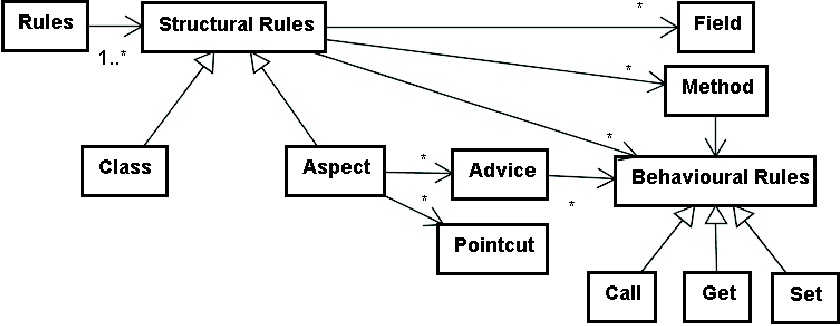
\includegraphics[width=1.0\textwidth]{images/meta-model}\\
%%  \caption{Design Rule Language and Configuration Module Meta-Models}\label{fig:meta-model}
%%  \end{center}
%%\end{figure}
%
%Figure~\ref{fig:meta-model}(a) shows the Design Rules
%specification language meta-model. A rule description is composed
%by one or more structural rules. They are used to define
%structural constraints for classes and aspects. Thus, a class can
%define fields, method signatures and behavioral rules. This
%behavioral rule can be defined within classes and aspects scope or
%within methods and advices. When a behavioral rule is defined
%within the scope of a class or aspect it means that it has to be
%executed at any place, for example, if a rule \emph{call} is used
%within the scope of a class means that the required method must be
%called at least once in any place this class. The
%Figure~\ref{fig:meta-model}(b) depicts the configuration module
%meta-model used to describe a configuration option of the
%specified components by Design Rule. The configuration module
%define which components will follow a particular structural rule
%(\emph{Declaration}) and which parameters (\emph{Parameter}) are
%informed.
%
%For simplicity we do not detail the parametrization mechanism in
%this model. This mechanism can be used to parameterize the method
%signature and fields. For example, we can use the rule
%\emph{set(field)} to allow that a particular field is updated.
%This field could be parameterized and the concrete value would be
%specified by configuration module.

\section{Evaluation}

% Discuss the benefits of applying the DR language in different case studies
% - Health watcher
% - choose one of the cases: TaRGeT, Games, Mobile Media, FLIP, \ldots
% Evaluate the benefits based on metrics
% - Concern metrics or Lattix Metrics

In this section we evaluate our language for specifying design rules
in AO systems. Basically, we discuss advantages and disadvantages of
using our approach when compared to other ones like Crosscutting
Programming Interfaces (XPIs). In what follows, we describe the
details of our evaluation:

%\begin{itemize}
%    \item[$\square$] hhh
%    \item[$\square$] aaa
%\end{itemize}

\subsection{Auditing Concern}

The auditing concern must be triggered when inserting, removing,
updating, or searching for a complaint.

Two teams working in parallel without design rules: the first one
works on the base code (the ComplaintRepository) and the second one
works on the auditing concern. Such a concern is implemented as an
aspect.

\scriptsize
\begin{lstlisting}[frame=single, caption={Complaint Repository implementation.},label=lst:complaint-repository, language=Java]
public class ComplaintRepository implements IComplaintRepository {

    public int insert(Complaint c) throws RepositoryException,
            ObjectAlreadyInsertedException {

    }

    public void update(Complaint c) throws RepositoryException,
            ObjectNotFoundException {

    }

    public void remove(int id) throws RepositoryException,
            ObjectNotFoundException {

    }

    public Complaint search(int id) throws RepositoryException,
            ObjectNotFoundException {

    }

}
\end{lstlisting}
\normalsize

Aspect for implementing the auditing concern:

\scriptsize
\begin{lstlisting}[frame=single, caption={Auditing Aspect.},label=lst:auditing-aspect, language=Java]
public aspect AuditingAspect {

    pointcut auditWhen():
           execution(int ComplaintRepository.insert(Complaint)
        || execution(void ComplaintRepository.update(Complaint)
        || execution(void ComplaintRepository.remove(int)
        || execution(Complaint ComplaintRepository.search(int)

    after() returning(): auditWhen() {
        // audit code.
    }

}
\end{lstlisting}
\normalsize

In the meanwhile, suppose that the teams are working on their
respective concerns (the repository and the auditing concerns). Now,
suppose that the team of the repository changes the following:

\begin{itemize}
    \item the insert method returns void instead of int; and

    \item the remove and search methods should take as parameter the
    Complaint object instead of an id.
\end{itemize}

Such changes might break the aspects...

% =================================== at� aqui entraria na se��o 2...

% ===== se��o 4

Design Rule:

\scriptsize
\begin{lstlisting}[frame=single, caption={Auditing Design Rule.},label=lst:auditing-dr, language=Java]
dr AuditingDesignRule {

    class ComplaintRepository {

        public int insert(Complaint c) throws RepositoryException,
                ObjectAlreadyInsertedException {}

        public void update(Complaint c) throws RepositoryException,
                ObjectNotFoundException {}

        public void remove(int id) throws RepositoryException,
                ObjectNotFoundException {}

        public Complaint search(int id) throws RepositoryException,
                ObjectNotFoundException {}

    }

    aspect AuditingAspect {

        pointcut auditWhen():
            execution(int ComplaintRepository.insert(Complaint)
            || execution(void ComplaintRepository.update(Complaint)
            || execution(void ComplaintRepository.remove(int)
            || execution(Complaint ComplaintRepository.search(int)

        % precisa do args aqui...??? Acho que sim...

        after() returning(): auditWhen() {
            xcall(void Auditing.auditComplaint(Complaint));
        }

    }

}
\end{lstlisting}
\normalsize

XPI of this example:

\textbf{Observa��o para colocar no texto: a XPI garante que n�o h�
chamadas fora do aspecto. No entanto, ela n�o garante:}

\begin{itemize}
    \item Que ocorre realmente uma chamada para auditComplaint;
    \item O local exato dessa chamada (dentro de um aspecto, por exemplo).
\end{itemize}

\scriptsize
\begin{lstlisting}[frame=single, caption={Auditing XPI.},label=lst:auditing-xpi, language=Java]
public aspect AuditingXPI {

    pointcut auditWhen():
        execution(int ComplaintRepository.insert(Complaint)
        || execution(void ComplaintRepository.update(Complaint)
        || execution(void ComplaintRepository.remove(int)
        || execution(Complaint ComplaintRepository.search(int)

    pointcut callToAudit(): call(void Auditing.auditComplaint(Complaint));

    declare error: (callToAudit() && !within(AuditingXPI)):
        "Contract violation: the auditComplaint method can not
        be called outside the aspect AuditingXPI";

}
\end{lstlisting}
\normalsize

In order to guarantee the contract that classes, aspects and their
respective methods and advices must exist, we can informally
document it like a prose, as mentioned in~\cite{sss}. Obviously, in
this case the contract is not verified by using the AspectJ
compiler, for instance.

However, we can guarantee the aforementioned contract by using
Aspect-Aware interfaces~\cite{sss}. Figure TAL illustrates that when
a pointcut does not match any piece of code, the compiler emits a
warning to the developer. Such a warning might be used to alert the
developer that some method must exist, for example.

\textbf{Observa��o para colocar no texto:}

As marca��es de AJDT (did not match) pode nos ajudar a identificar
classes ou m�todos que n�o existem. Mas elas n�o ajudam a
identificar que determinados aspectos ou advices existem.

Com quantifica��o, a AJDT consegue fazer as marca��es. No entanto,
ao remover um join point que � capturado pelo aspecto, nenhum erro �
apresentado (ou seja, n�o h� garantias que um determinado join point
existe ou n�o).

\subsection{Transaction Concern}

All methods of the HealthWatcherFacade must have transaction
management. In this case, due to the crosscutting nature of this
concern throughout the methods, we can use aspects to modularize it,
as showed in Listing TAL.

\scriptsize
\begin{lstlisting}[frame=single, caption={Transaction Management Aspect.},label=lst:transaction-aspect, language=Java]
public aspect HWTransactionManagement {

    pointcut transactionalMethods(): execution(* HealthWatcherFacade.*(..));

    after() returning: transactionalMethods()  {
        // ta errado... n�o � a interface
        IPersistenceMechanism.commitTransaction();
    }

    after() throwing: transactionalMethods()  {
        IPersistenceMechanism.rollbackTransaction();
    }

    before(): transactionalMethods() {
        IPersistenceMechanism.beginTransaction();
    }

}
\end{lstlisting}
\normalsize

\subsection{Concurrency Concern}

Section TAL showed the concurrency concern implemented as an aspect.
All methods of the \emph{EmployeeRepository} were synchronized by
the \emph{SynchronizationAspect}. In what follows, we present design
rules and XPIs to avoid modularity problems.

\scriptsize
\begin{lstlisting}[frame=single, caption={Concurrency Design Rule.},label=lst:concurrency-dr, language=Java]
dr Concurrency {

    class EmployeeRepository {

    }

    aspect SynchronizationAspect {

        pointcut concurrency(): execution(* EmployeeRepository.*(..));

        Object around(): concurrency() {

        }

    }

}
\end{lstlisting}
\normalsize

\subsection{Product Line Games}

\section{Concluding Remarks}

% a summary of the main concluding remarks 
% of the paper.



\bibliographystyle{abbrv}
\bibliography{jss2008}


\end{document}